 Two lines passing through the point(2,3) intersect each other at an angle of $60\degree$.If slope of one line is 2,find equation of the other line.

\textbf{Solution :}

\begin{table}[H]
    \centering
    \begin{tabular}{|c|c|c|}
    \hline
        \textbf{Symbol} &\textbf{Description}&\textbf{Value}  \\
        \hline
         $m_1$&Slope of one line &2\\
         \hline
         $m_2$&Slope of another line&$m$\\
         \hline
         $\vec{P}$&Intersecting point&$\myvec{
             2\\3
         }$\\
         \hline
         $\theta$&Angle between two lines&$60\degree$\\
         \hline
    \end{tabular}


    \caption{Table of input parameters}
    \label{tab:11.10.3.12.1}
\end{table}



\begin{table}[H]
    \centering
    \begin{tabular}{|c|c|c|}
    \hline
        \textbf{Symbol} &\textbf{Description}&\textbf{Value}  \\
        \hline
         $\vec{m_1}$&Direction vector of one line&$\myvec{
             1\\2
         }$\\
         \hline
         $\vec{n_1}$&Normal vector of one line&$\myvec{
             2\\-1
         }$\\
         \hline
        $\vec{m_2}$&Direction vector of another line&$\myvec{
             1\\m
         }$\\
         \hline
          $\vec{n_2}$&Normal vector of another line&$\myvec{
             m\\-1
         }$\\
         \hline
    \end{tabular}


    \caption{Table of output parameters}
    \label{tab:11.10.3.12}
\end{table}


So,
\begin{align}
  \cos{60\degree}&=\frac{\vec{\brak{m_1^T}m_2}}{\vec{\norm{m_1}\norm{m_2}}}\\
    or,\frac{1}{2}&=\frac{\myvec{
        1&2
    }\myvec{
        1\\m
    }}{\sqrt{5}\sqrt{m^2+1}}\\
   or, \frac{1}{2}&=\frac{1+2m}{\sqrt{5m^2+5}}\\
   or,11m^2+16m-1&=0\\
   or, m&=\frac{-8\pm5\sqrt{3}}{11}    
\end{align}
Therefore,the direction vector is,$\vec{m_2}=\myvec{
    1\\\frac{-8+5\sqrt{3}}{11}
}$ or,$\myvec{
    1\\\frac{-8-5\sqrt{3}}{11}}$

The normal vector is,$\vec{n}=\myvec{
    \frac{-8+5\sqrt{3}}{11}\\-1
}$or,$\myvec{
    \frac{-8-5\sqrt{3}}{11}\\-1
}$

So, the equation of the line is
\begin{align}
\vec{n^Tx}=c\\
\myvec{
    \frac{-8\pm5\sqrt{3}}{11}&-1
}\vec{x}&=c
\end{align}
Passes through the point $\vec{P}=\myvec{
    2\\3}$
\begin{align}
\myvec{
    \frac{-8\pm5\sqrt{3}}{11}&-1
}\vec{P}=c\\
 or,c=\frac{-49\pm16\sqrt{3}}{11}
\end{align}


\textbf{Figure :}
\begin{figure}[H]
    \centering
    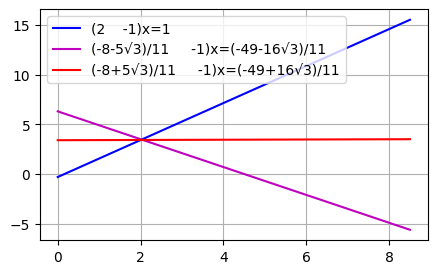
\includegraphics[width=\columnwidth]{chapters/11/10/3/12/fig/asgnt1.png}
    \caption{}
    \label{fig:11.10.3.12}
\end{figure}

